\chapter{Introduction}
\label{chapter:intro}
%The opening paragraph should motivate the central theme of the thesis. Exaplain what the core problem is, and why that's important. Bear in mind that this chapter is targeting a broard audience, so try to be as accessible as possible. 

Decision trees \cite{breiman2001random} and deep learning \cite{lecun2015deep} have become ubiquitous in the field of medical image processing. With the combination of the increasing volume of digitised imaging data and advances in both hardware and software,  these so-called ``black-box" machine learning (ML) algorithms have enabled a substantial leap in performace in a plethora of applications from image analysis to surgical assistance \cite{criminisi2013decision,litjens2017survey}. For certain well-defined tasks with access to homogeneous and carefully annotated data, such machine learning systems have begun to surpass the performance of clinical experts \cite{esteva2017dermatologist,gulshan2016development,rajpurkar2017chexnet,wu2019deep}. However, translation of these research innovations into clinical practice requires care. In medical imaging applications where the algorithm's outputs inform scientific conclusions in research, and diagnostic, prognostic or interventional decisions in clinics, we need principled protocols to ensure safety. 

In practice, ML systems often face situations where the correct decision or prediction is ambiguous. We therefore need a mechanism to quantify the confidence of the model output (e.g. error bounds) and act upon it to prevent catastrophic failures. We would also like to be able to reason about the sources of such uncertainty, and further improve the performance. Does the training data need to be more diverse? Were the images or the annotations too noisy? It might have been that the choice of the model was not adequate. Or perhaps we may have been just unlucky and the particular instance of failures is an inherently challenging case where the input image did not contain enough information. Implementing systematic approaches to answering these questions is important not only to improve the predictive performance, but also to build trust with the practioners. However, to date, the majority of deep learning and decision tree techniques used in the medical imaging context rely on deterministic methods, and lack a mechanism to communicate uncertainty, a key ingredient to address such problems. 

In contrast, \textit{probabilistic machine learning} provides a natural framework to quantify the degree of uncertainty over different variables of interest, be it the prediction, the model parameters and structures, or the underlying data (images and labels) \cite{ghahramani2015probabilistic}. Probability distributions are used to represent all the uncertain unobserved quantities in a model and how they relate to the data, and probability theory is used as a language to compute and manipulate these distributions. The main goal of this thesis is to develop a practical framework for medical imaging applications to model and reason under different types of uncertainty in neural networks and decision trees by translating ideas from the paradigm of probabilistic machine learning. In the process, several fundamental enhancements to current methods arise. 

\textcolor{red}{\textbf{Could include a couple of illustrative failure cases? } }



%The most widely used deep learning models have an important shortcoming: they lack an under- lying mechanism to provide uncertainty infor- mation about the predictions they make. Instead they often output point estimates between 0 and 1, which are often taken blindly as a measure of confidence. There have already been a few high profile cases where blindly trusting deci- sions made by deep learning algorithms has had disastrous consequences. For example in 2016, and then again in 2018, there were fatalities due to mistakes made by the perception system of autonomous vehicles. In health care a wrong decision can be a matter of life or death, and so being able to place trust in the decisions of deep learning models applied to such an industry is of critical importance.

% These questions are becoming more important to patient safety as many research groups and companies have deployed or are aiming to deploy ML technology in clinical practice.
%
%
% In practice, ML systems often face situations where the correct decision is ambiguous, and therefore principled mechanisms for quantifying uncertainty are required to envision potential practical deployment.

%
%
%
%\paragraph{Deep learning and decisions trees are ubiquitous in research:} 
%\begin{itemize}
%	\item Decision trees and deep learning have become ubiquitous in the field of medical image processing. The combination of the increasing volume of digitised imaging data and advances in both hardware and software enabled these high-performance machine learning models have lead to substantial progress in a wide range of applications ranging from image analysis to surgical assistance. 
%	\item Super-human performance for well-defined tasks when a large volume of clean data is available. 
%	\item Deployment in practice requires safety. Decting when the model fails. 
%\end{itemize}
%
%
%\paragraph{The importance of uncertainty quantification}
%\begin{itemize}
%	\item Many of the above problems are characterised by uncertainty. 
%	\item Probability theory provides a language for manipulating and representing these different types of uncertainty. 
%\end{itemize}
%
%\paragraph{Over-realiance on deterministic algorithms. }
%\begin{itemize}
%	\item To date, the current methods disproportionately focus on the performance and rely on deterministic algorithms. 
%	\item The central theme of the thesis to investigate ways to reason about different forms of uncertainty and assess the utility in different medical imaging applications.  
%\end{itemize}
%



%	\begin{enumerate}
%		\item The omission of clinical-practice guidelines produced a machine learning algorithm suggesting that respiratory infections are a leading cause of chest pain, completely omitting cardiac causes
%		\item An algorithm developed to help detect melanoma, for instance, should be derived from a sufficiently diverse sample; when these data aren’t used or aren’t available, algorithms run the risk of overlooking disease in underrepresented patient populations. 
%		\item Clinically important variables and endpoints should be present and robust, but this remains a challenge in many data resources. 
%\end{enumerate} }
%\textcolor{red}{\textbf{Explain through an example to illustrate the importance of uncertainty modelling?
%Quantifying risks, understand the sources of uncertainty and point to solutions. Pneumonia risk prediction? }}


%Deep learning and decisions trees are now ubiquitous in the field of medical image processing. However, the current methods disproportionately rely on deterministic algorithms, which lack a mechanism to represent and manipulate uncertainty about models and predictions. In safety-critical applications such as medical imaging, quantifying what the model does not know is important for constructing a reliable decision making system. The aim of this thesis is to explore probabilitic modelling as a framework to integrate uncertainty information in deep learning and decision tree models, and demonstrate utility in various medical image processing applications. 
%
%\textcolor{red}{
%	I should end with a clear goal statement. Examples from two notable theses are below:
%	\begin{itemize}
%		\item (David Mackay): ``The main goal of this thesis is to provide an objective and practical framework for the use of neural network techniques by applying the methods of Bayesian model comparison. In the process several enhancements to current neural network methods arise.''
%		\item (Yarin Gal): ``The main goal of this thesis is to develop such practical tools to reason about uncertainty in deep learning.''
%\end{itemize}}

 \section{Taxonomy of Uncertainty}
There are many different types of uncertainty that are of practical importance. Here we provide a taxonomy of such uncertainty ``species'' as illustrated in Fig.~\ref{fig:uncertainty_taxonomy} and explain their relations and differences. 

Imagine you have a machine learning model, $F_{\theta}$, which takes some input $\mathbf{x}$  (e.g. a MR image) and makes a prediction or decision, $\hat{\mathbf{y}}=F_{\theta}(\mathbf{x})$, about the quantity of interest, $\mathbf{y}$ (e.g. presence of pathology). Here we use different notations, $\mathbf{y}$ and $\hat{\mathbf{y}}$, to emphasize the difference between the target output variable and its estimate from the model. In this case, $\theta$ denotes the parameters of the model, and has been optimised based on training data, consisting of $N$ pairs of inputs and labels of interest $\mathcal{D} = \{\mathbf{x}_{i}, \mathbf{y}_i\}_{i=1}^N $. You now have thoroughly evaluated the performance on a held-out test dataset (e.g. a large public imaging dataset), and are about to deploy it in the wild (e.g. your local hospital).

\textit{Predictive uncertainty} describes the degree of ambiguity (or confidence) in the model's prediction on an given input. For example, error bounds are a common measure of predictive uncertainty, and can be used to assess the reliability of prediction for the particular data instance at hands. You might be interested in knowing how well your model performs in a new environment, but you may not have access to a sufficient volume of ground-truth labels for validation. However, quantification of predictive uncertainty provides a proxy measure of performance on each data point, which can be used to manage failure risks in a principled way---if the model encouters input examples with overly high predictive uncertainty, then we should not trust the system. 

One is often interested not only in quantifying the predictive uncertainty, but also understanding its \textit{sources}. Having quantitative answers to questions such as ``is the model uncertain on this particular image because the observed feature is not represented in the training data or the image quality is too low to make definitive decisions? Perhaps the current model does not best explain the data and we should use a different one?'' has clear benefits for building a more realiable system. Commonly, such \textit{source} uncertainty is divided into two types, \textit{aleatoric} and \textit{epistemic} uncertainty \cite{hora1996aleatory,der2009aleatory}. 

\textit{Aleatoric uncertainty} --- from the Latin word, \textit{alea}, meaning a ``die'' --- refers to uncertainty inherent to a problem that in principle cannot be reduced by additional physical or experimental knowledge. For example, the mapping from input $\textbf{x}$ to target $\mathbf{y}$ which one wants to approximate from data may be intrinsically stochastic. For example, an acquired image $\textbf{x}$ does not contain enough information to conclude whether an observed feature is pathological or not, and thus both predictions ``pathology is present'' and ``pathology is absent'' are equally probable. Such inherent ambiguity is only worsened by the fact that the training data $\mathcal{D}$ may be corrupted by observational noise (such as measurement errors and annotation noise).  

\textit{Epistemic uncertainty} — from the Greek word \textit{episteme}, meaning “knowledge” — refers to uncertainty arising from lack of knowledge. In the context of modelling, epistemic uncertainty is often subdivided into \textit{parameter uncertainty}, in which one believes that the form of the model reflects reality well, but one is uncertain about which values of the parameters $\theta$ in the model to use, and \textit{structural uncertainty}, in which one has significant doubts that the model $F_{\theta}(\cdot)$ is even ‘structurally correct’ (e.g. is linear regression appropriate or a neural network, if the latter, how many layers, etc).


\begin{figure}[ht]
	\vspace{-2mm}
	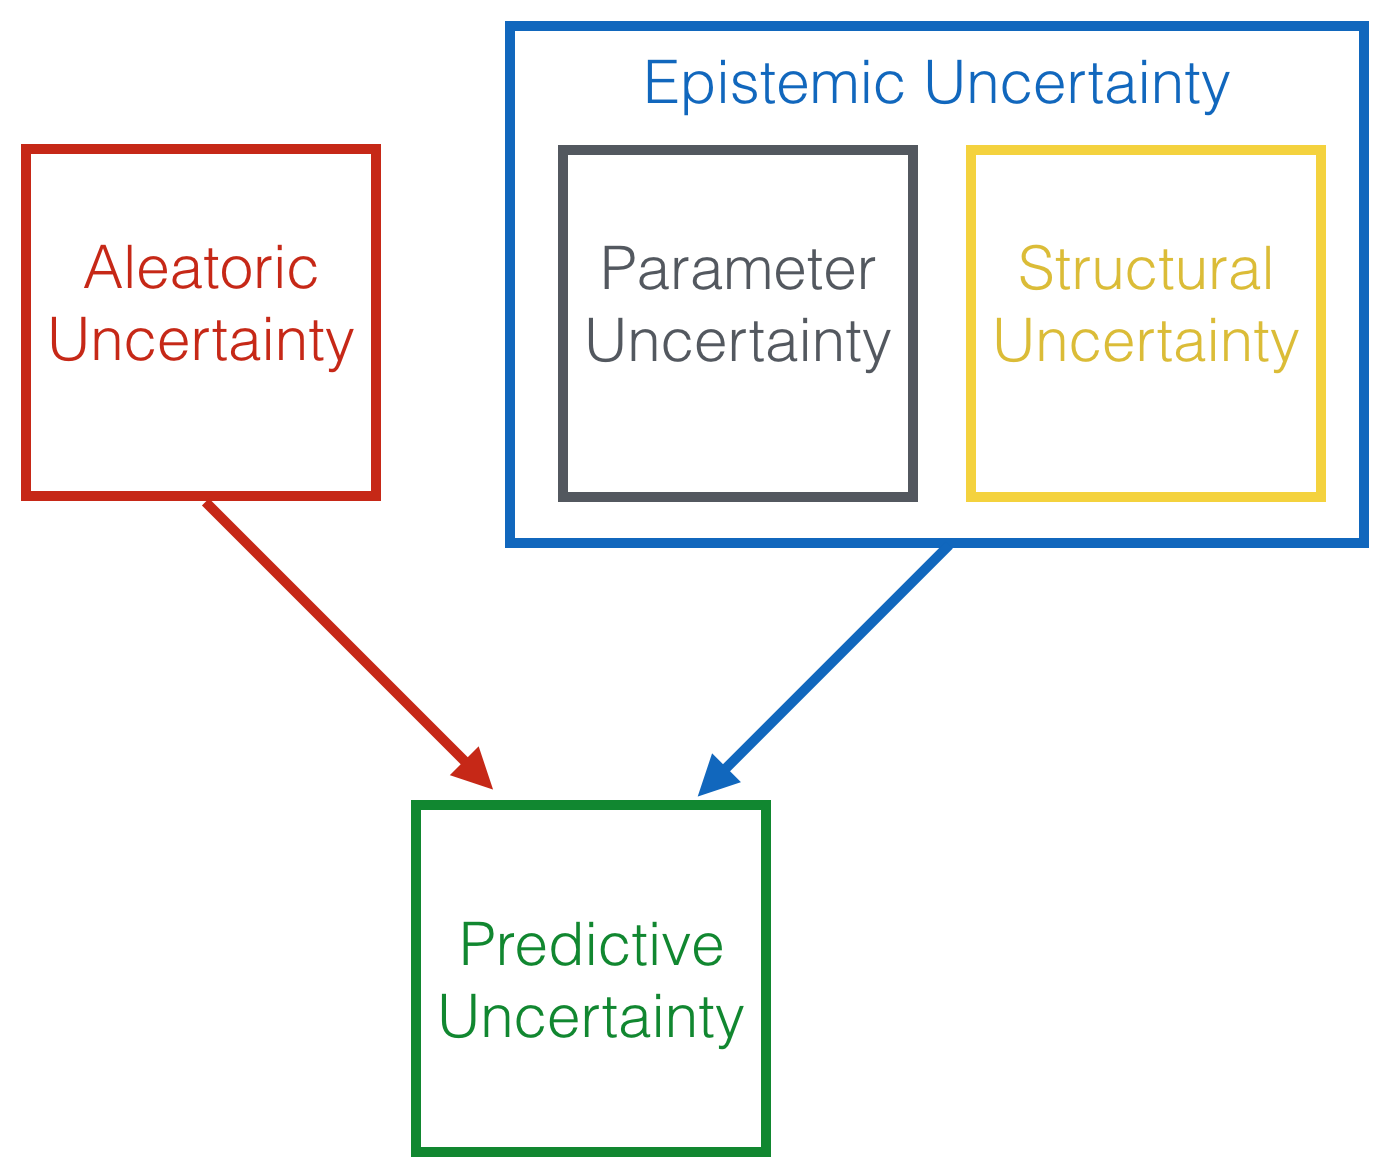
\includegraphics[width=0.4\linewidth]{chapter_1/uncertainty_taxonomy.png}
	\centering	
	\vspace{-2mm}
	\caption{\small Illustration of different types of uncertainty. The combined effects of both aleatoric and epistemic uncertainties induce \textit{predictive uncertainty}.  } 
	\label{fig:uncertainty_taxonomy}
	%\vspace{-10pt}
\end{figure}

We should, however, note that the distinction between epistemic and aleatoric uncertainty is a rather ambiguous one and depends somewhat on the interpretation of what probability means \cite{cox2006principles,samaniego2010comparison}. For example, an orthodox frequentist, who believes in the definition of a probability based on the objective relative frequency of events, would say that the results of a coin flip are random and represents aleatoric uncertainty.  On the other hand, a devout Bayesian, who believes probabilites represents degrees of subjective ignorance, might say that the coin flip is characterised by epistemic uncertainty, arguing one is simply ignorant about the set of influential parameters e.g. initial conditions of the coin such as the angle and height of the drop, the material and shape of the coin, and the dynamics of the wind which may affect the trajectory, etc. In any case, putting aside the details of philosophical debates surrounding such categorisation of uncertainty, the language of probability theory provides a powerful tool in describing different forms of uncertainty \cite{sullivan2015introduction}. This thesis, in particular, focuses on the ways to describe such uncertainty with(in) deep learning and decision tree models, and aims to demonstrate their practical benefits in medical imaging applications. 

In the probabilistic framework of machine learning, all uncertain quanitities are treated as random variables, and 
probability distributions are used to express their associated information of uncertainty. For example, the aleatoric uncertainty of the target mapping $\textbf{x} \rightarrow \mathbf{y}$ is summarised by the underlying conditional distribution of the task $P(\mathbf{y}|\mathbf{x})$. This distribution describes the inherent stochasticity in predicting $\mathbf{y}$ for input $\mathbf{x}$. On the other hand, the parameter uncertainty is described by $P(\theta|\mathcal{D}, m)$, the posterior distribution over the unknown parameters $\theta$ of the model class $m=\{F_{\theta}(\cdot): \theta \in \Theta\}$ given the training observations $\mathcal{D}$. Similarly, strucutural uncertainty is described by the distribution $P(m|\mathcal{D})$ which quantifies how probable the model class explains the observations. Finally, the predictive uncertainty is represented in the conditional distribution $P(\hat{\mathbf{y}}|\mathbf{x})$ over the model's output $\hat{\mathbf{y}}=F_{\theta}(\mathbf{x})$, and its standard deviation is commonly used as a confidence interval. The technical problems tackled in this thesis boil down to the estimation of these distributions in different settings. As will be explained later, for complex models such as deep neural networks and decisions trees, many of these distributions are not tractable, necessitating efficient and effective approximations. 

To make matters even worse, in practical applications such as medical imaging, the ground truths for such distributions of interest, $P(\mathbf{y}|\mathbf{x}), P(\hat{\mathbf{y}}|\mathbf{x}), P(\theta|\mathcal{D}, m)$ and $P(m|\mathcal{D})$ are not available, thus rendering the direct evaluation of uncertainty estimation unfeasible. In this thesis, I take a pragmatic position and focus on evaluating the utility---rather than the fidelity---of the derived uncertainty estimates via surrogate measures, such as the generalisation to out-of-distribution data and domain, robustness to noise and biases, detection of unseen structures, certification of performance with confidence intervals, etc. 

%To provide more precise definitions of the aforementioned types of uncertainty, we assume that the data generating process is untouchable\footnote{This is hardly realistic in the context of science.} and we only have freedoms in the way to describe the data (i.e. models). Under this assumption, we can separate 
%We further confine 

%The combined effects of these disparate sources of aleatoric and epistemic uncertainties induce predictive uncertainty described above as diagrammed in Fig.~\ref{fig:uncertainty_taxonomy}. Decompoding the overall measure of predictive uncertainty into such orthogonal sources 


%The probabilistic approach to modelling uses probability theory to express all forms of uncertainty [9]. Probability theory is the mathematical language for representing and manipulating uncertainty [10], in much the same way as calculus is the language for representing and manipulating rates of change. Fortunately, the probabilistic approach to modelling is conceptually very simple: probabil- ity distributions are used to represent all the uncertain unobserved quantities in a model (including structural, parametric, and noise-related) and how they relate to the data. Then the basic rules of probability theory are used to infer the unobserved quantities given the observed data. Learn- ing from data occurs through the transformation of the prior probability distributions (defined before observing the data), into posterior distributions (after observing data). The application of probability theory to learning from data is called Bayesian learning (Box 1)”
 
%Taking a pragmatic point of view and declining the related philosophical debates, the use of probability theory for either uncertainty is a common modeling choice in UQ.

%In statistical inference, frequentist and Bayesian approaches differ in the way they address these uncertainties  

%Someone who was simultane- ously a devout Newtonian physicist and a devout Bayesian might argue that the results of dice rolls are not aleatoric uncertainties — one simply doesn’t have complete enough information about the initial conditions of die, the material and geometry of the die, any gusts of wind that might affect the flight of the die, and so forth. On the other hand, it is usually clear that some forms of uncertainty are epistemic rather than aleatoric: for example, when physicists say that they have yet to come up with a Theory of Every- thing, they are expressing a lack of knowledge about the laws of physics in our universe, and the correct mathematical description of those laws. In any case, regardless of one’s favoured interpretation of probability, the language of probability theory is a powerful tool in describing uncertainty.


 
%The model may encouter some unfamiliar inputs, which are not observed in the training data (e.g. a rare pathology).
% 

 
%More abstractly, the below are the types of uncertainty that the prior methods have tried to account for: 
%\begin{itemize}
%	\item Aleatory (intrinsic) uncertainty
%	\item Parameter uncertainty. 
%	\item Structural uncertainty. 
%\end{itemize}



% (From Sullivan 2015): It is common to divide uncer- tainty into two types, aleatoric and epistemic uncertainty. Aleatoric uncer- tainty — from the Latin alea, meaning a die — refers to uncertainty about an inherently variable phenomenon. Epistemic uncertainty — from the Greek ε`πιστη ́μη, meaning knowledge — refers to uncertainty arising from lack of knowledge. If one has at hand a model for some system of interest, then epis- temic uncertainty is often further subdivided into model form uncertainty, in which one has significant doubts that the model is even ‘structurally correct’, and parametric uncertainty, in which one believes that the form of the model reflects reality well, but one is uncertain about the correct values to use for particular parameters in the model

%Different areas of applications in medical imaging have studied to varying degrees ways to represent these types of uncertainty, which I elaborate in the remaining part of this section. 
%
%\textcolor{red}{Explain more fundamentally how probabilistic modelling provides a language to manipulate uncertainty about models and predictions. Read Zoubin's paper? This would be more of a background materials though. I guess we could come up with a very simple example to illustrate all these aspects? Perhaps augment Zoubin's example?}




\section{Uncertainty Modelling in Medical Imaging}
% I would like to use this section to motivate the importance of uncertainty quantification in medical imaging applications. 
The importance of representing uncertainty information has long been recognised in the medical imaging community before the recent surge of deep learning methods. There is a large body of prior research on uncertainty quantification, based on traditional probabilistic machine learning techniques in a variety of medical image processing tasks such as classification, registration, segmentation and synthesis. Here I provide a brief survey of such prior arts. 
  
 % (Yarin says): This probabilistic view of machine learning offers confidence bounds for data analysis and decision making, information that a biologist for example would rely on to analyse her data, or an autonomous car would use to decide whether to brake or not. In analysing data or making decisions, it is required to be able to tell whether a model is certain about its output, being able to ask “maybe I need to use more diverse data? or change the model? or perhaps be careful when making a decision?”. Such questions are of fundamental concern in Bayesian machine learning, and have been studied extensively in the field [Ghahramani, 2015]. 
 
% (Mackay says:) Bayesian probability theory provides a framework for inductive inference which has been called ‘common sense reduced to calculation’; it is a poorly known fact that Bayesian methods actually embody Occam’s razor automatically and quantitatively [26, 38].

\subsection{Classification} 
Many medical decisions can be viewed as classification tasks where the information about patients are used as inputs to infer some discrete states of their health (e.g. diagnosis) and the subsequent course of treatment (e.g. prognosis). It is widely accepted that the information available to the physician about her patient and about medical relationships in general is inherently uncertain. Since the advent of computers, academics have attempted to formalise and emulate the process of such medical reasoning performed under uncertainty,  in an attempt to support clinicians through systemisation and standardisation of knowledge. Ledley et al. \cite{ledley1959reasoning} proposed in the 1950s the first decision theoretic framework to aggregate medical evidence of varying degrees of uncertainty, and derive the most likely diagnosis in a restricted setting. They introduced scoring cards for doctors to represent the presence of discriminative symptoms, and designed an automatic system to process them to compute the conditional probability of the disease of interest. During the subsequent twenty years from then, more advanced computerised diagnostic systems were developed for different problems \cite{shortliffe1979knowledge,kulikowski1980artificial,duda1983expert}, however, most were still manually designed and deterministic rule-based systems without a mechanism to account for uncertainty. Adlassing et al. \cite{adlassnig1985cadiag,adlassnig1986fuzzy} employed `fuzzy set theory' to quantify and reason with ambiquities which arise in each local decision of the if–then-else statement within such decision trees, which improved accuracy and robustness in applications in internal medicince\footnote{Incidentally, a recent study \cite{berner2008overconfidence} showed that over-confidence of doctors is also a big cause of diagnostic errors in medicine!}. Specifically, both the objective uncertainty of each decision measured in frequency of past occurence, and the subjective uncertainty based on the confidence of practioner were integrated to infer the plausibility of different diagnostic outcomes. More recently, the above approach was augmented with a variety of pre-processing steps to learn fuzzy rules automatically from data \cite{steimann1998fuzzy,john2005modeling,straszecka2006combining,anooj2012clinical,tsipouras2008automated}. 

Another popular alternative to the above rule-based approaches is based on Bayesian networks (BNs) \cite{pearl2014probabilistic}. A typical BN-based decision model consists of a set of nodes and edges with directions, where the nodes are random variables which represent a set of symptoms and diseases, and the directed edges define the probabilistic relationships (conditional dependencies) between them, which can be more complex than the simple if-then-else conditional statements. In addition to such generality, BNs are attractive because they can naturally communicate the uncertainty in possible diagnostic alternatives as well as its underlying compositional reasoning even when data is incomplete or partially correct \cite{nikovski2000constructing}. Some notable applications of BNs include the diagnosis of cardiovascular diseases from echocardiography \cite{diez1997diaval}, prediction of mental retardation in newborn babies \cite{mani1997mentor}, classification of ,  detection of breast cancer in mammography \cite{kahn1997construction,sajda2003multi,burnside2004probabilistic}. A more extensive review of the existing research, including attempts to mine unknown causal structures between symptoms and diseases, are provided in Sec.~2 in Luiz et al \cite{seixas2014bayesian}. Some of such development have also gone beyond the realm of academic research; several computerised diagnosis (also known as computer-aided diagnosis (CAD) \cite{doi1993digital}) systems have been approved by FDA for mammographic screening  and used in clinical practice \cite{sajda2006machine}. 


%Bayesian networks have been broadly applied in biomedicine, particularly in probabilistic expert systems for clinical diagnosis (96–98) and computational biology (99). They are attractive because they are able to deal with biomedical data that is incomplete or partially correct (100). A novel method for exploiting conditional dependencies in the structure of radiological images to improve detection of breast cancer is described below.

%Better classification accuracy is not enough for an expert system to be used in practice.It must be able to explain its decisions and it must be flexible enough to provide all possible alternatives.

\subsection{Registration}
Image registration is the problem of determining a geometric transformation to establish spatial correspondences between images. This task plays a foundational role in numerous image-guided medical tasks \cite{maintz1998survey,glocker2011deformable,sotiras2013deformable} performed in both research and clinics. Firstly, it allows the spatial normalisation of multiple subjects into a common reference frame---often referred to as inter-subject registration---which is an important pre-processing step for population modeling of anatomical variability. Secondly, registration can also be used to align images of the same subject---referred to as intra-subject registration---acquired at (i) different time points or (ii) different imaging devices. The former is crucial for longitudinal studies where temporal structural or anatomical changes are examined, while the latter aims to fuse information from multiple imaging modalities to facilitate diagnosis and treatment planning. 

However, specification of the optimal alignment suffers from significant uncertainty due to the ill-posed nature of the problem, presence of imaging artifacts, and the inherent variability of human anatomy. The most established approach to combat such ambiguity is probabilistic registration techniques \cite{van2008encoding,risholm2010summarizing,cobzas2011random,lotfi2013improving,simpson2012probabilistic,risholm2013bayesian,popuri2013variational,zhang2013bayesian,wassermann2014probabilistic,simpson2015probabilistic,heinrich2016deformable,le2016quantifying} where the process of registration is modelled as a hierarchical generative model, and the inference yields an estimation of the posterior distributions over the parameters of both regularisation and transformation models. These techniques, not only enhance the performance of registration by automatically tuning the level of regularisation on the given data, but also enable ones to derive measures of registration uncertainty from the estimated distribution of possible transformations, which can be accounted for in dowstream tasks.

Probabilistic registration methods can be broadly categorised into two classes, depending on whether the space of transformation is modelled as discrete \cite{cobzas2011random,popuri2013variational,heinrich2016deformable} and continuous \cite{van2008encoding,simpson2012probabilistic,risholm2013bayesian,zhang2013bayesian,wassermann2014probabilistic,simpson2015probabilistic,le2016quantifying} random variables. The associated registration uncertainty are typically quantified by summary statistics of such transformation distributions (e.g., the Shannon entropy in the discrete case \cite{lotfi2013improving}, and the variance \cite{simpson2012probabilistic,le2016quantifying}, standard deviation\cite{simpson2015probabilistic} or inter-quantile range \cite{risholm2013bayesian,risholm2010summarizing} in the continuous case), and are visualised on top of the registerred image as a surrogate measure of registration accuracy, which is difficult to measure in practice. Some works have also demonstrated the utility of uncertainty measures in dowstream tasks such as dose estimation in radiotherapy \cite{risholm2011estimation}, segmentation of human brains \cite{simpson2011probabilistic} and classification tasks where features are derived from spatially normalised images \cite{simpson2012ensemble}. Luo et al. \cite{wells2018miccai}, however, recently has pointed to a glitch in the treatment of registration uncertainty in the existing research, highlighting the discrepancy between the  uncertainty over transformations and the uncertainty over the output registerred image, which is of real practical interest. 
%The prior research have attempted to account for such ambiguity of the task to design a more robust method 


%an uncertainty measure that highlights loca- tions where the algorithm had diculty finding a proper alignment can be very helpful. 


% Secondly, registration can be used to align images of the same subject, known as intra-subject registration. These images may have been acquired at di↵erent times, or using different imaging modalities. As such, intra-subject registration provides a mechanism for describing anatomical changes in a subject over time. Both inter-subject and intra-subject registration are explored in this thesis.
%
%
%The spatial alignment such as population modeling and longitudinal studies, and computer-assisted diagnosis and interventions. 

 %Image registration has a broad variety of medical applications [84], and has been implemented using a wide range of methodologies (see [121][207] for reviews)


%\textbf{(Wells 2018 MICCAI)}: ``Probabilisitc image registration (PIR) literature conventionally quantifies the registration un- certainty by summary statistics of the transformation distribution. Previous researchers have found applications of various summary statistics: the Shannon entropy and its variants of the categorical transformation distribution were used to measure the registration uncertainty of DPR [6]; the variance [4,11,13], stan- dard deviation [10], inter-quartile range [5,15] and the covariance Frobenius norm [9] of the transformation distribution were used to quantify the registration un	certainty of CPR.''
%
%\textbf{(Chapter 6 in Ivor Simpson's thesis):} "Registration Derived Uncertainty" describes how the uncertainty could be used in the downstream tasks. 

\subsection{Segmentation}
Image segmentation has been, along with image registration, one of the main challenges in modern medical image analysis, and describes the process of assigning each pixel or voxel in images with biologically meaningful discrete labels, such as anatomical structures and tissue types (e.g. pathology and healthy tissues). The task is required in many clinical and research applications, including surgical planning \cite{gering2001integrated,mazzara2004brain}, and the study of disease progression, aging or healthy development \cite{fischl2002whole,prastawa2005automatic,zijdenbos2002automatic}. However, there are often cases in practice where the correct delineation of structures is truly uncertain; this is also reflected in the well-known presence of high inter- and intra-reader variability in segmentation labels obtained from trained experts \cite{warfield2004simultaneous,joskowicz2018automatic,joskowicz2019inter}. 

The vast majority of probabilistic segmentation methods model such uncertainty in pixel-wise manner, estimating the probability vector over classes in each pixel. Such approaches often fall into the categorty of either discrimative or generative approaches, although some hybrid models also exist \cite{heckemann2006automatic,tu2008brain,iglesias2011combining,criminisi2011discriminative}. In the former,  

Tumours: Probabilistic boosting trees \cite{wels2008discriminative}, Naive Bayes classifier 
Brain: AdaBoost \cite{morra2008automatic}
Pulmonary emphysema: \cite{prasad2008multi}
Organs: random forest \cite{criminisi2009decision}



while in the latter, 


reflected by the high variability amon



Eugnio mentioned in his paper 2013 \cite{iglesias2011combining} that "most approaches to joint segmentation of multiple structures rely on registration (i.e. by deforming an atlas (or a set thereof) to the target scan)". A very different approach from the mindless end-to-end learning that's so prevalent nowadays!  

(\textbf{Need to read}): Karl Friston's unified segmentation paper, Eugenio's MCMC based segmentation paper, and 

\textbf{(Claudia Blaiotta): } "One of the most significant advantages of variational inference over maximum likelihood estimation is its intrinsic capability of containing the effects of overfitting (Attias, 1999; Bishop, 2006). In the case of mixture models this allows, for instance, determining the optimal number of components (K) without performing cross-validation, which is usually rather demanding for the amount of computation, as well as for the amount of data, that it requires (Bishop, 2006)."

See Sec 5.2. (Page 106) "Advantages and challenges of Bayesian inference” where she comments that 
"In practice, this also means that explicit confidence measures cannot be directly obtained for the estimated parameters, which is a significant drawback for potential clinical applications, where the risk of error or failure needs to be accurately assessed and quantified.” 

Read "Juan Eugenio Iglesias, Mert Rory Sabuncu, and Koen Van Leemput. Incorporating parameter uncertainty in Bayesian segmentation models: Application to hippocampal subfield volumetry. In Proc. International Conference on Medical Image Computing and Computer Assisted Intervention, MICCAI 2012, pages 50–57. Springer, 2012b. "

(Zach ER): "While it remains uncommon to calculate estimates of uncertainty in probabilistic segmentation – indeed, many methods preclude it entirely – Bayesian models of segmentation incorporate estimates of model parameter variance explicitly, and even downstream errors such as volume estimates [1]. These methods have however seen limited adoption: they are computationally expensive, especially compared with modern CNNs, and have worse accuracy. In addition, the formulation in [1] relies on having a probabilistic atlas to use as a prior term, which may not be amenable to highly variable pathological tissues such as tumours or Multiple Sclerosis lesions."

%(Eugnio) The probabilistic perspective, with its flexibility and principled in- ference machinery, offers another promising direction for future re- search. In particular, this approach enables the derivation of meth- ods that can handle missing labels, heterogeneous labels, variable imaging modalities, estimate and utilize model uncertainty, and in- tegrate domain knowledge, for example about the anatomy or imag- ing physics. Furthermore, probabilistic algorithms offer the capability to quantify the uncertainty in the final segmentation estimate, which can further be utilized for obtaining more accurate measurements, for example of the volume of structures (Iglesias et al., 2013a).

\subsection{Synethesis}
Jorge's paper and Nichola's ayaches' work. 

\subsection{Inverse Problems}
\textcolor{red}{(2019-Aug-22): This may take some time. Perhaps skip for now and come back.}
\begin{itemize}
	\item Reconstruction
	\item Deblurring, denoising, dealiasing, super-resolution 
\end{itemize}


\section{What is lacking?}
Having motivated the importance of modelling uncertainty in medical imaging, now I would like to give a brief account on the recent successes of decision trees and deep learning, the classes of machine learning models that this thesis focuses on. 

In the last few years, discriminative approaches based on these powerful non-linear models have permeated the field of medical image processing \cite{criminisi2013decision,shen2017deep,litjens2017survey}, surpassing the performance of more traditional probabilistic techniques in well-defined problems with abundant labelled data. Beyond the automation of existing radiological tasks--- e.g. segmentation \cite{kamnitsas2017efficient}, detection \cite{roth2014new}, disease grading and classification \cite{araujo2017classification}---deep learning has been applied to a diverse set of ``data enhancement'' problems. Data enhancement aims to improve the quality, the information content, or the quantity of medical images available for research and clinics by transforming images from one domain to another \cite{isola2017image}. Previous research has shown the efficacy of data enhancement in different forms such as super-resolution \cite{oktay2016multi,chen2018efficient,ravi2019adversarial}, image synthesis \cite{nie2016estimating,kang2017deep}, denoising \cite{benou2017ensemble,chen2017low}, data harmonisation \cite{karayumak2018harmonizing,tax2019cross} across scanners and protocols, reconstruction \cite{sun2016deep,jin2017deep,hammernik2018learning,schlemper2018deep,zhu2018image,yang2018dagan,yoon2019efficient}, registration \cite{sokooti2017nonrigid,balakrishnan2018unsupervised} and quality control \cite{wu2017fuiqa,esses2018automated}.  These advances have the potential not only to enhance the quality and efficiency of radiological care, but also facilitate scientific discoveries in medical research through increased volume and content of usable data. 

However, despite the surge of interest in the last couple of years (cite some recent methods including my work?),  it still remains that the disproportionate majority of approaches rely on deterministic methods, which lack a mechanism to represent and manipulate uncertainty about models and predictions. In safety-critical applications such as medical imaging, quantifying what the model does not know is important for constructing a reliable decision making system. The aim of this thesis is to explore probabilitic modelling as a framework to integrate uncertainty information in deep learning and decision tree models, and demonstrate utility in various medical image processing applications. 

\textcolor{red}{The aim of the thesis is to investigate ways to } 

 
\section{Progress in Probabilistic Decision Trees and Deep Leanring}
This section will review theoretical research on uncertainty modelling in deep learning and decision trees. We will discuss why such research is important for designing safe and interpretable systems for medical applications. 

\textcolor{red}{This thesis is a mixture of applications of these methods to practical medical imaging problems, and development of new methods building upon such work. }


\section{Contributions} 
\textcolor{red}{Until the late 2015 (around when my PhD started), no methods specifically had attempted address the problem of uncertainty quantification with decision trees and deep neural networks. The presence of this gap, combined with the rising interest in the use of these powerful ``black-box" approaches, motivated me to explore this topic in a variety of settings, with an eye on the eventual utilty in medical applications. More specifically, the contributions of this thesis can be recapitulated as follows:}

\begin{enumerate}
	\item \textbf{Modelling predictive uncertainty}:  We introduce methods to quantify uncertainty over the output of deep learning and decision tree models. We demonstrate how such uncertainty measure can be used to quantify the quality of output and develop a more risk-averse image enhancement system for diffusion MRI \cite{tanno2016bayesian,tanno2017bayesian,tannonimg2019}.  We further show that the same concept could be naturally extended to the multi-task learning paradigm, and test the benefits in the context of MR-only radiotherapy planning application \cite{bragman2018multi}. 
	
	\item \textbf{Modelling structural uncertainty}: We propose methods to learn model structures of a deep neural network. In the context of multi-task learning, we introduce the concept of \emph{stochastic filter  groups} (SFGs) \cite{sfg2019} to estimate the posterior distribution over the possible connectivity structures in a convolutional neural network in order to disentangle task-specific and shared features across different tasks. We demonstrate in the MR-only radiotherapy planning application that SFGs are capable of learning meaningful separations of representations, and consequently improve the performance. Lastly, we explore how the training algorithm of decision trees could be extended to adapt the architecture of a neural network to the given availability of training data and the complexity of the task \cite{AdaptiveNeuralTrees19}. 
	
	\item \textbf{Modelling human uncertainty}: We propose a method to model the biases and skill levels of human annotators, and integrate this information into the learning process of the neural network classifier \cite{tanno2019learning}. We demonstrate in classification of ultrasound cardiac images that the method not only improves the robustness of the model to label noise, but also yields insights into the performance of different human annotators.
	
\end{enumerate}

\section{Thesis Structure}
The thesis outline is as follows. In Chapter~\ref{chapter:biqt}, we introduce a probabilistic variant of decision trees to quantify predictive uncertainty, and demonstrate on image enhancement of neuroimages. In Chapter~\ref{chapter:deepuncertainty}, we focus on the same application, but explore ways to estimate the uncertainty over the prediction of deep learning models. We design a framework to jointly model the aleatoric uncertainty of the target mapping of interest, and the parameter uncertainty of the model, and propagate the two to estimate the predictive uncertainty. In Chapter~\ref{chapter:multitaskuncertainty_part1}, we show that the same concept could be naturally adapted to the multi-task learning paradigm, and demonstrate the benefits in the MR-only radiotherapy treatment planning application where the synthetic CT image and the segmentation of organs at risk are simultaneously predicted from the input MR image. Motivated by the same problem, Chapter~\ref{chapter:multitaskuncertainty_part2} introduces a Bayesian method to learn the connectivity structures in a neural network. The goal here is to disentangle task-specific and shared features across different tasks, and thereby benefit more from jointly learning from multiple related talks. In Chapter~\ref{chapter:ant}, we explore how the training algorithm of decision trees could be extended to learn the structure and the complexity of a network architecture for the given availability of data and the complexity of the task. In Chapter~\ref{chapter:humanuncertainty}, we consider explicitly modelling the ``measurement noise'' of human annotators, and propose a well-grounded and practical optimisation method to learn such noise model. We evaluate the method in the cardiac view classification task of ultrasound images, where the annotations are very noisy and sparse. Finally, in Chapter~\ref{chapter:conclusions}, we make overall conclusions, discuss the application of this technology and suggest directions for future research. For each chapter’s topic, we review the relevant prior art. 

\section{The road not taken}
\textcolor{red}{\textbf{Technical scope:} Here I should try and limit the scope by clearly explaining that the thesis focuses on simple supervised discriminative models, while touching upon other important avenues of research i.e.  generative, marriage between discriminative and generative, reinforcement learning (?), etc. We could use Eugenio's this year's MICCAI paper as a good example of hybrid models. }

\textcolor{red}{\textbf{Application scope:}  should also mention that the thesis focuses on tasks of processing high-dimensional image data that arise in medical settings. However, in fact, healthcare domain offers much richer array of data such as sensors, genomics, EHRs, and etc \cite{esteva2019guide}, which are outside the scope of the thesis. This link also has a few relevant references \href{https://www.mckinsey.com/industries/pharmaceuticals-and-medical-products/our-insights/machine-learning-and-therapeutics-2-0-avoiding-hype-realizing-potential}{link}.}

\section*{Publications}
\small
\begin{enumerate}
	\item \textbf{R. Tanno}, A. Ghosh, F. Grussu, E. Kaden, A. Criminisi, and D. C. Alexander, “Bayesian image quality transfer". (2016) \textbf{MICCAI}
	
	\item \textbf{R. Tanno}, D. E. Worrall, A. Ghosh, E. Kaden, S. N. Sotiropoulos, A. Criminisi, and D. C. Alexander, “Bayesian image quality transfer with cnns: Exploring uncertainty in dmri super-resolution”. (2017) \textbf{MICCAI}
	
	\item D. C. Alexander, D. Zikic, A. Ghosh, \textbf{R. Tanno}, V. Wottschel, J. Zhang, E. Kaden, T. B. Dyrby, S. N. Sotiropoulos et al., “Image quality transfer and applications in diffusion MRI”.  (2017) \textbf{Neuroimage}
	
	\item \textbf{R. Tanno}, A. Makropoulos, S. Arslan, O. Oktay, S. Mischkewitz, F. Al-Noor1, J. Oppenheimer, R. Mandegaran, B. Kainz, M. Heinrich. ``AutoDVT: Joint Real-time Classification for Vein Compressibility Analysis in Deep Vein Thrombosis Ultrasound Diagnostics''. (2018) \textbf{MICCAI}
	
	\item F.J.S. Bragman, \textbf{R. Tanno}, Z. Eaton-Rosen, W. Li, D. J. Hawkes, S. Ourselin, D. C. Alexander, J. R. McClelland, M. J. Cardoso, ``Uncertainty in multitask learning: joint representations for probabilistic MR-only radiotherapy planning''. (2018) \textbf{MICCAI}
	
	\item S. B. Blumberg, \textbf{R. Tanno}, I. Kokkinos, D. C Alexander. ``Deeper Image Quality Transfer: Training Low-Memory Neural Networks for 3D Images''. (2018) \textbf{MICCAI }
	
	\item K. Kamnitsas, D. Castro, L. Folgoc, \textbf{R. Tanno}, D. Rueckert, B. Glocker, A. Criminisi, A. Nori. ``Semi-Supervised Learning via Compact Latent Space Clustering''. (2018) \textbf{ICML}
	
	\item \textbf{R. Tanno}, A. Saheedi, S. Sankaranarayanan, D. C. Alexander, N. Silberman, ``Learning From Noisy Labels By Regularized Estimation Of Annotator Confusion''.  (2019) \textbf{CVPR}
	\item \textbf{R. Tanno}, K. Arulkumaran, D. C. Alexander, A. Criminisi and A. Nori,  “Adaptive Neural Trees”.  (2019) \textbf{ICML }
	\item F.J.S. Bragman$^*$, \textbf{R. Tanno}$^*$, S. Ourselin, D. C. Alexander, M. J. Cardoso, ``Stochastic Filter Groups for Multi-Task CNNs: Learning Specialist and Generalist Convolution Kernels''.  (2019) \textbf{ICCV} ($^*$ equal contributions)
	
	\item \textbf{R. Tanno}, D. E. Worrall, E. Kaden, A. Ghosh, F. Grussu, A. Bizzi, S. N. Sotiropoulos, A. Criminisi, and D. C. Alexander, ``Uncertainty Quantification in Deep Learning for Safer Neuroimage Enhancement''. (2019) \textbf{Neuroimage} (Under Submission)
	
	\item F.J.S. Bragman$^*$, \textbf{R. Tanno}$^*$, S. Ourselin, D. C. Alexander, M. J. Cardoso, ``Learning task-specific and shared representations in medical imaging''.  (2019) \textbf{MICCAI} ($^*$equal contributions)
	
	\item C. Sudre, B.G. Anson, S. Ingala, D. Jimenez, C. Lane, L. Haider, T. Varsavsky,  \textbf{R.~Tanno}, L. Smith, S. Ourselin, R. Jager, M. J. Cardoso, ``Let's agree to disagree: learning highly debatable multirater labelling''.  (2019) \textbf{MICCAI} 
	
	\item S. B. Blumberg, M. Palombo, C. S. Khoo, C. Tax, \textbf{R. Tanno}, D. C Alexander. “Multi-Stage Prediction Networks for Data Harmonization”. (2019) \textbf{MICCAI }
	
	\item K. Quan, \textbf{R. Tanno}, M. Duong, R. Shipley, M. Jones, C. Bereton, J. Hurst, D. Hawkes, J. Jacobs, 	``Modelling Airway Geometry as Stock Market Data using Bayesian Changepoint Detection'', (2019) \textbf{MICCAI} 10$^{\text{th}}$Machine Learning in Medical Imaging Workshop
	
\end{enumerate}

\newpage
\section*{Patents}
\begin{enumerate}
	\item  \textbf{R. Tanno}, K. Arulkmaran, A. Nori, A. Criminisi, “Neural Trees”, G.B. Microsoft Technology Licensing LLC. (2018). Patent No. GB201810736D0. (Filed in Aug 2018).
	\item F. A. Noor, S. Mischkewitz, A. Makropoulos, \textbf{R. Tanno}, B. Kainz, O. Oktay, “Blood vessel obstruction diagnosis method, apparatus \& system”  Patent No.WO2018162888A1. (Published in Sep 2018).
	
\end{enumerate}

